\section{Linguagem Java}
Java é considerada a linguagem de programação orientada a objetos mais utilizada no Mundo, base para a construção de ferramentas como Hadoop, Pentaho, Weka e muitas outras utilizadas comercialmente. Foi desenvolvida na década de 90 por uma equipe de programadores chefiada por \textit{James Gosling} para o projeto Green, na Sun Microsystems - tornou-se nessa época como a linguagem que os programadores mais baixaram e o sucesso foi instantâneo. Em 2008 o Java foi adquirido pela Oracle Corporation.

\subsection{Driver JDBC de Conexão}
Para proceder a conexão com Java, é necessário baixar um driver JDBC (Java Database Connection). Existem vários drivers construídos. Para utilizar o driver é necessário criar um projeto (vamos usar o \textbf{Spring Tool Suite 4}, utilize se quiser qualquer outro editor de sua preferência).

No STS4 acessar a seguinte opção no menu: File $\triangleright$ New $\triangleright$ Java Project. Informar o nome do projeto (Decus), não esquecer de modificar a opção "Use an environment JRE" para a versão correta da Java Runtime desejada e pressionar o botão Finish.

Agora devemos convertê-lo para um projeto Apache Maven. Clicar com o botão direito do mouse no projeto e acessar a opção: Configure $\triangleright$ Convert to Maven Project. Na janela apenas pressione o botão \textit{Finish}. Se tudo está correto observamos que o projeto ganhou uma letra \textbf{M} o que indica agora é um projeto padrão Maven. Então foi criado um arquivo chamado \textbf{pom.xml}. 

Acessar este arquivo e antes da tag BUILD, inserir a tag DEPENDENCIES:
\begin{lstlisting}[]
<dependencies>
  <dependency>
    <groupId>redis.clients</groupId>
    <artifactId>jedis</artifactId>
    <version>2.8.1</version>
  </dependency>
</dependencies>
\end{lstlisting}

Agora a situação do projeto é esta:
\begin{figure}[H]
	\centering
	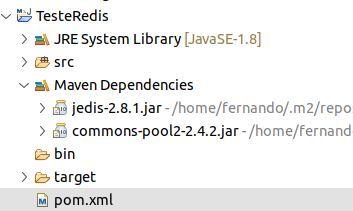
\includegraphics[width=0.5\textwidth]{imagens/dependenciasMaven}
	\caption{Dependências do Maven}
\end{figure}

Observamos que na pasta \textbf{Maven Dependencias} foi baixado a versão 2.8.1 do driver Jedis - Isso não é erro de digitação realmente o driver se escreve com "J".

\subsection{Exemplo Prático de uma Escola}
Estamos prontos para testarmos a conexão entre Redis e Java. Criamos um pequeno exemplo que nos auxiliará como teste, uma classe chamada \textbf{Escola} no pacote \textbf{decus.com} e inserimos nesta a seguinte codificação:
\begin{lstlisting}[]
package decus.com;

import java.text.SimpleDateFormat;
import java.util.Date;
import redis.clients.jedis.Jedis;

public class Escola {
	
 private String [] materias = new String[] {
  "Matemática Computacional", "Programação", "Estatística",
  "SQL", "NoSQL", "Java", "Python", "Análise de Dados",
  "Arquitetura de DW", "Big Data"
 };
 public static void main(String [] args) {
  new Escola().executar();
 }
 private void executar() {
  adicionarNotas();
 }
}
\end{lstlisting}

Nossa escola promove cursos mensais e temos um conjunto contendo todas as matérias que são aplicadas aos alunos. Ao término do curso é registrado o nome do aluno, a matéria e sua nota. Escolhemos o Redis para conter esses dados exatamente devido a sua característica de chave-valor.

No método principal que chama o executar, em Java não devemos programar no método "main". No executar colocamos uma chamada ao método criarAlunos() que terá a seguinte codificação:
\begin{lstlisting}[]
private void adicionarNotas() {
 Jedis jedis = new Jedis();
 String data = new SimpleDateFormat("dd/MM/yyyy").format(new Date());
 String chave = "";
 String [] nomes = new String[] {
  "Alice", "Miguel", "Sophia", "Arthur", "Helena", "Bernardo", "Valentina", 
  "Heitor", "Laura", "Davi", "Isabella", "Lorenzo", "Manuela", "Théo", "Júlia", 
  "Pedro", "Heloísa", "Gabriel", "Luiza", "Enzo", "Maria", "Luiza", "Matheus", 
  "Lorena", "Lucas", "Lívia", "Benjamin", "Giovanna", "Nicolas", "Maria", 
  "Eduarda", "Guilherme", "Beatriz", "Rafael", "Clara", "Joaquim", "Cecília"
 };
 String nome = "";
 for (int i = 0; i < 50; i++) {
  nome = nomes[(int)(Math.random()*nomes.length)] + " " + nomes[(int)(Math.random()*nomes.length)];
  for (int j = 0; j < materias.length; j++) {
   chave = "MAT" + i + "-" + j + "-" + data;
   jedis.hset(chave, "nome", nome);
   jedis.hset(chave, "materia", materias[j]);
   jedis.hset(chave, "nota", ""+(int)(Math.random()*11));
   jedis.close();
  }
 }
 System.out.println("Notas Adicionadas");
}
\end{lstlisting}

Obviamente como isto é um simples exemplo vamos adicionar as notas de uma forma totalmente aleatória.

Neste método temos a definição do objeto do Jedis que é responsável pela comunicação com o banco de dados que deve estar disponível na porta padrão. Criamos duas listas de nomes e matérias apenas para compor as notas que iremos inserir e ter dados mais elaborados. Teremos 50 alunos que ganharão nomes e sobrenomes completamente aleatórios com base na primeira lista, para cada um deles percorremos a lista de matéria e definimos uma chave que será composta por: "MAT" + valor de i (que é o número do aluno) + valor de j (que é o número da materia) e a data que estamos inserindo a informação. Assim temos a garantia que essa chave será única.

Para inserir a informação no objeto Jedis temos o método "hset" que recebe 3 parâmetros a chave, o nome do campo e o valor deste, e assim inserimos os campos nome, matéria e nota que será obtida também de forma aleatória (entre o valor de 0 a 10). Uma vez executado temos como resposta na console a mensagem "Notas Adicionadas" se verificamos no aplicativo "Another Redis Desktop Manager" teremos os seguintes dados:
\begin{figure}[H]
	\centering
	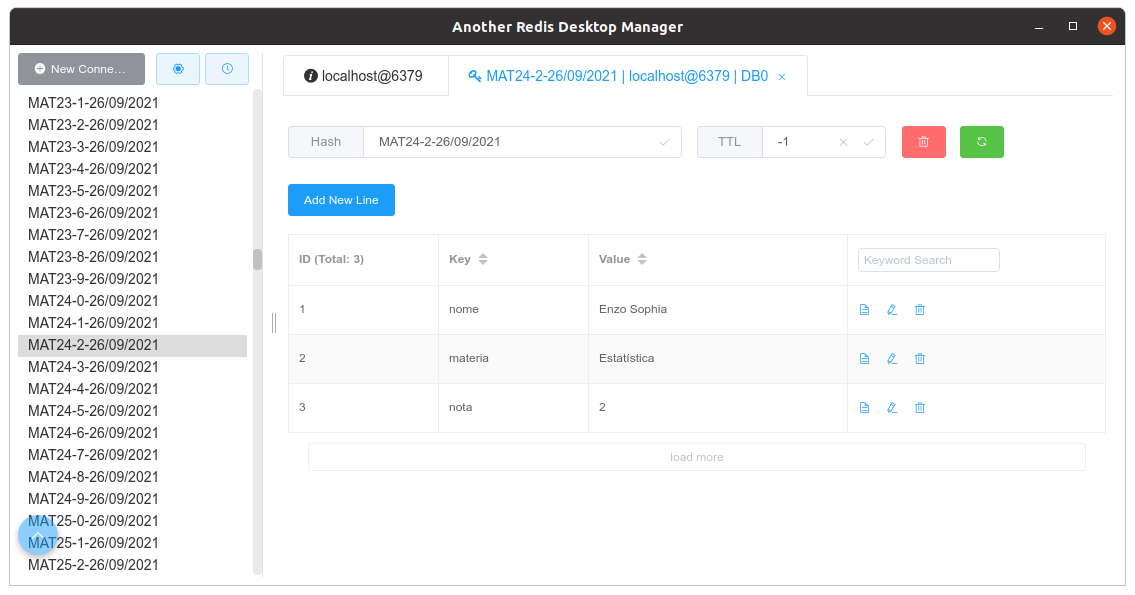
\includegraphics[width=0.7\textwidth]{imagens/notasAlunos}
	\caption{Another Redis Desktop Manager}
\end{figure}

Obviamente que os dados podem dar diferença pois o nome e as notas foram selecionados randomicamente.

\subsection{Localizações}
No método executar comentamos a chamada ao método "adicionarNotas()" e criamos outra para o método "trazerAluno(1)" que terá a seguinte codificação:
\begin{lstlisting}[]
private void trazerAluno(int mat) {
 Jedis jedis = new Jedis();
 Set<String> nomes = jedis.keys("MAT" + mat + "-*");
 java.util.Iterator<String> it = nomes.iterator();
 String s;
 while (it.hasNext()) {
  s = it.next();
  System.out.print(jedis.hget(s, "nome") + " - ");
  System.out.print(jedis.hget(s, "materia") + " - ");
  System.out.println(jedis.hget(s, "nota"));
 }
 jedis.close();
}	
\end{lstlisting}

As coisas no Redis são bem fáceis e rápidas, recebemos a matrícula e obtemos um conjunto (objeto Set) com todas as chaves que começam pela expressão "MAT1-" (como o valor que passamos foi 1) podemos utilizar esse método para realizar qualquer tipo de pesquisa, por exemplo "*-26/09/2021" trará todas as chaves do dia "26/09/2021". 

Percorremos esse conjunto e obtemos os dados que desejamos através do método "hget" no qual passamos a chave e o campo que desejamos. Ao executarmos teremos na console o nome do aluno, o nome da matéria e a nota obtida por esse.

Mas e se por exemplo desejamos saber a média geral das matérias dessa turma em cada matéria? Comentamos a chamada ao "trazerAluno(1)" no método executar por "mediaGeral()" e adicionamos a seguinte codificação:
\begin{lstlisting}[]
private void mediaGeral() {
 Jedis jedis = new Jedis();
 String materia = "";
 for (int i = 0; i < materias.length; i++) { 
  int totNota = 0;
  int qtdNota = 0;
  Set<String> nomes = jedis.keys("*-"+i+"-*");
  java.util.Iterator<String> it = nomes.iterator();
  String s;
  while (it.hasNext()) {
   s = it.next();
   materia = jedis.hget(s, "materia");
   totNota += Integer.parseInt(jedis.hget(s, "nota"));
   qtdNota++;
  }
  System.out.println(materia + " - " + (totNota/qtdNota));
 }
 jedis.close();
}	
\end{lstlisting}

E temos na saída da console cada uma das matérias e sua respectiva média.

\subsection{Eliminar Registro}
Assim como a consulta do registro é obtida através da chave o mesmo se aplica para a eliminação do mesmo, vamos comentar a chamada ao método "mediaGeral()" e chamar o método "eliminarAluno(1)" e adicionarmos a seguinte  codificação:
\begin{lstlisting}[]
private void eliminarAluno(int mat) {
 Jedis jedis = new Jedis();
 Set<String> nomes = jedis.keys("MAT" + mat + "-*");
 java.util.Iterator<String> it = nomes.iterator();
 String s;
 while (it.hasNext()) {
  s = it.next();
  jedis.del(s);
 }
 jedis.close();
 System.out.println("Notas Eliminadas");
} 	
\end{lstlisting}

Localizamos as chaves do aluno e executamos o método "del(chave)" para cada registro. Ou seja, extremamente simples e prático.

\subsection{Estrutura do objeto Jedis}
Aqui utilizamos o modelo estrutural de um Hash com mapeamento de um campo String como no de campo e seu respectivo valor e que pode ser aplicado para a grande maioria dos casos, porém existem outras estruturas no Redis que podem ser utilizadas com este conector.

\textbf{String}

É o modelo mais simples uma chave e um valor, pode ser utilizado por exemplo para uma associação de palavras como localidade e endereço:
\begin{lstlisting}[]
jedis.set("Joaquim Lucas", "Qd 28 Casa 47 Rua Amélia Cidade Vale Alegre");
jedis.set("Nicolas Cecília", "Qd 7 Casa 7 Rua Sete da Cidade Amarela");
System.out.println(jedis.get("Joaquim Lucas"));
\end{lstlisting}

Ou seja, utilizamos o método "set(chave, valor)" para inserirmos a informação e o método "get(chave)" para obtê-la. Esse modelo também pode ser utilizado como uma camada de cache extremamente rápida e simples de se usar para solicitações HTTP recebidas de um aplicativo Web ou outros requisitos de cache. 

\textbf{Listas}

São listas de strings, classificadas por ordem de inserção e podem ser uma ferramenta ideal para implementar, por exemplo, filas de mensagens:
\begin{lstlisting}[]
jedis.lpush("tarefas", "Primeira tarefa do dia");
jedis.lpush("tarefas", "Segunda tarefa do dia");
jedis.lpush("tarefas", "Terceira tarefa do dia");
\end{lstlisting}

A cada comando "lpush(chave, valor)" uma nova tarefa é inserida. Para retirar usamos o comando:
\begin{lstlisting}[]
System.out.println(jedis.rpop("tarefas"));
\end{lstlisting}

Devemos lembrar que precisamos serializar qualquer objeto e persisti-lo como uma string, portanto, as mensagens na fila podem transportar dados mais complexos quando necessário.

\textbf{Conjuntos}

Trata de uma coleção não ordenada de Strings e que são bem úteis quando desejamos excluir membros repetidos, para adicionar elementos usamos:
\begin{lstlisting}[]
jedis.sadd("frutas", "abacate");
jedis.sadd("frutas", "manga");
jedis.sadd("frutas", "abacate");

Set<String> conjunto = jedis.smembers("frutas");
System.out.println(jedis.sismember("frutas", "abacate"));
\end{lstlisting}

As frutas do Java Set terão um tamanho de 2, a segunda adição de "abacate" foi ignorada. O método sismember permite que verifiquemos a existência de um membro específico rapidamente e mesmo com a resposta "true" se olharmos no nosso banco (usemos o aplicativo "Another Redis Desktop Manager") veremos que só existe uma única ocorrência para "abacate".
\begin{figure}[H]
	\centering
	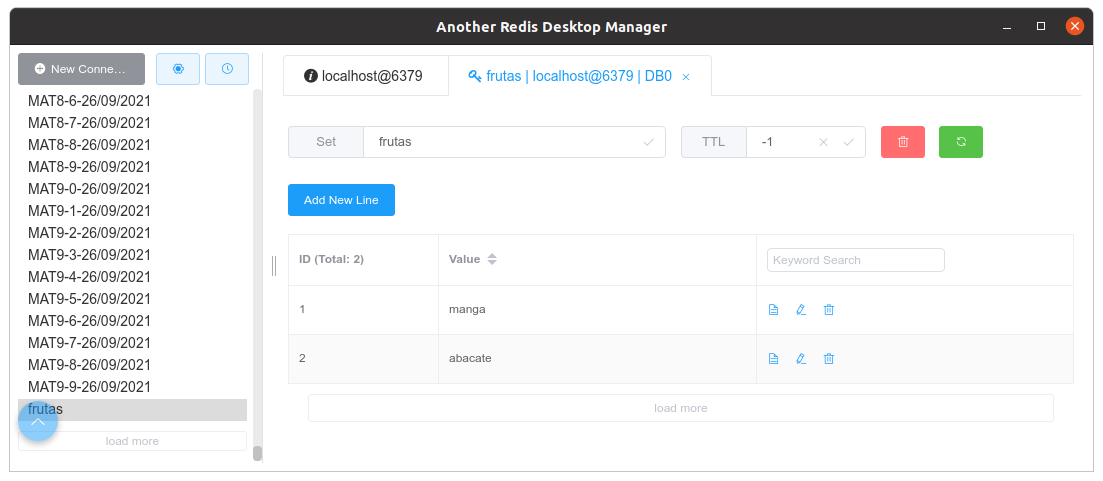
\includegraphics[width=0.8\textwidth]{imagens/frutas}
	\caption{Visão do Conjunto Frutas}
\end{figure}

\textbf{Conjuntos Ordenados}
São conjuntos classificados em que cada membro possui uma determinada classificação associada, que é usada para localizá-los. Podemos inserir alguns alunos e seus desempenhos da seguinte forma:
\begin{lstlisting}[]
Map<String, Double> desempenho = new HashMap<>();
desempenho.put("Aluno 1", 3000.0);
desempenho.put("Aluno 2", 1500.0);
desempenho.put("Aluno 3", 8200.0);
desempenho.put("Aluno 4", 2500.0);
desempenho.put("Aluno 5", 7500.0);
desempenho.put("Aluno 6", 6200.0);
desempenho.entrySet().forEach(playerScore -> {
  jedis.zadd("Desempenho", playerScore.getValue(), playerScore.getKey());
});	
\end{lstlisting}

E obtermos uma relação dos 3 melhores com a seguinte codificação:
\begin{lstlisting}[]
System.out.println("1o.: " + jedis.zrevrange("Desempenho", 0, 1).iterator().next());
System.out.println("2o.: " + jedis.zrevrange("Desempenho", 1, 2).iterator().next());
System.out.println("3o.: " + jedis.zrevrange("Desempenho", 2, 3).iterator().next());
\end{lstlisting}

Podemos utilizar de todas essas estruturas para criarmos uma aplicação extremamente veloz ou mesmo usar o Redis como um complementar para determinadas ações que precisamos aumentar os ganhos de velocidade.